% !TEX root = ../thesis.tex

\chapter{Problem Context}

In this chapter, the problem addressed in this master thesis is introduced, and an overview of the existing work is provided. The first section "FKIE" presents the scope of the problem and outlines the expectations of the \ac{IR} system from target users perspective. Subsequently, the definitions of several crucial keywords and technologies are provided in the section "Key Definitions". Additionally, the previous work conducted prior to this master thesis is discussed in the section named "Existing Work". Finally, "Problem Description" delves into the challenge in detail with presenting statistical information and discussing the potential of addressing the problem using well-established techniques.

	\section{FKIE}

The \ac{FKIE} is a renowned research institute dedicated to pioneering solutions in information and communications technology. Their primary focus lies in the development of effective and efficient human-machine systems\footnote{\url{https://www.fkie.fraunhofer.de/en/about-fkie.html}}. The users at \ac{FKIE} have a particular interest in accessing news articles that are related to  innovation and advancements in the fields of technology and military. \prettyref{fig:areas_of_interest} provides a visual representation of the areas of interest to the \ac{FKIE} users. It is important to note that this list is not bounded and can encompass additional domains.

\begin{figure}[h!]
	\centering
	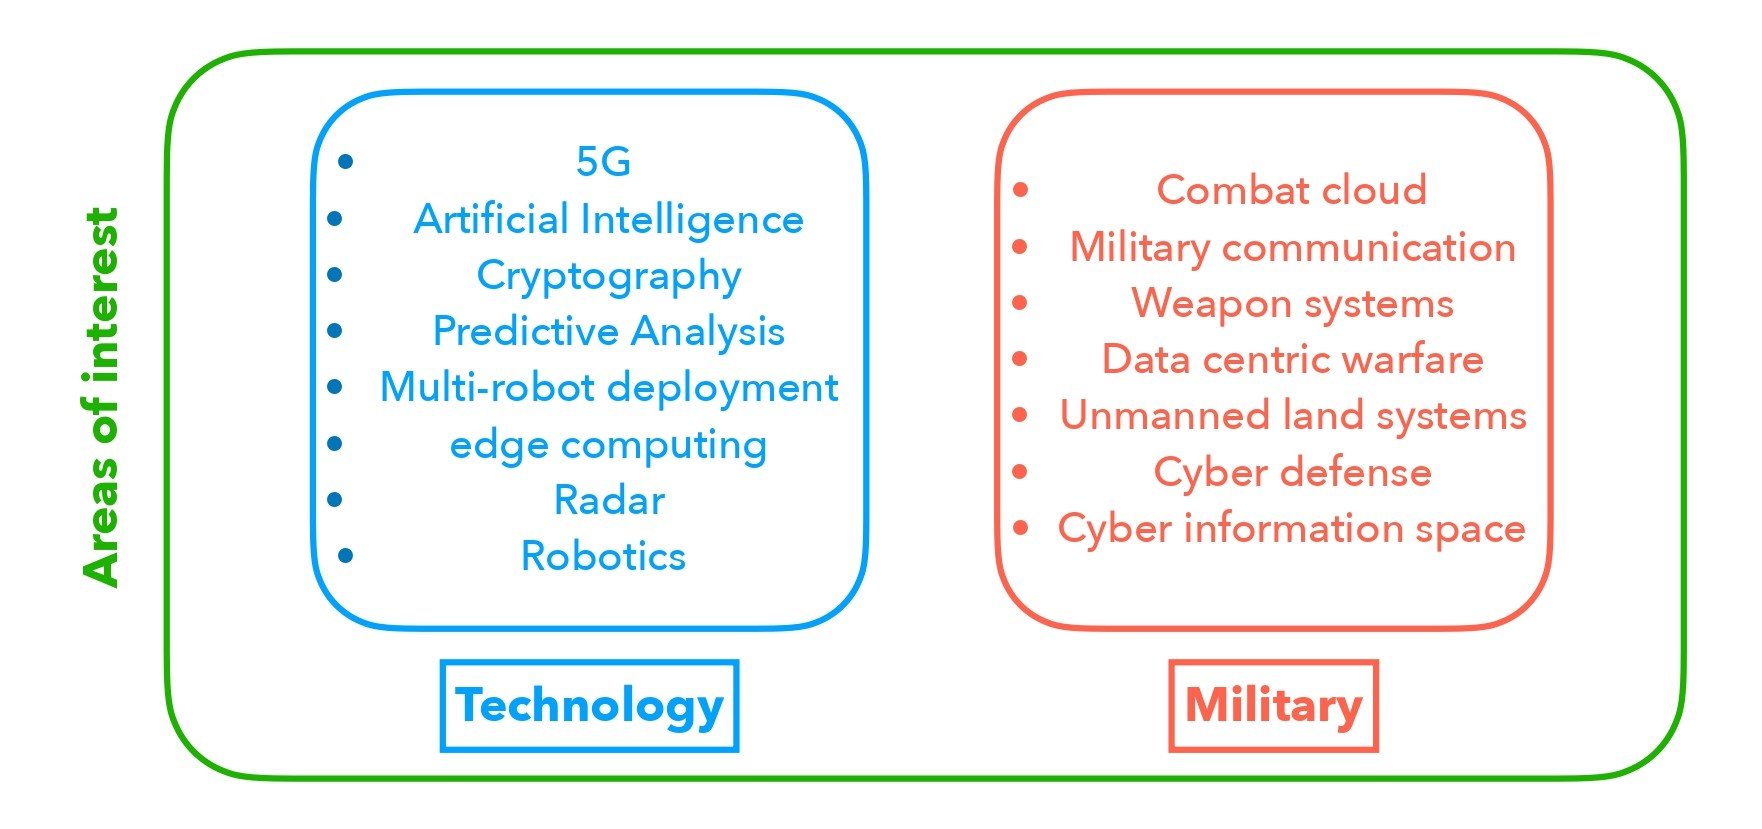
\includegraphics[width=.8\textwidth]{images/keynotes_images/areas_of_interest.jpg}
	\caption{Areas of interest for users at FKIE. \label{fig:areas_of_interest}}
\end{figure} 

\section{Key Definitions}

This section provides explanations of several key technologies utilized in the previous work and additional definitions can be found in Appendix \ref{appendix:A}.

\begin{description}
	
	\item[\ac{SVM}] \hfill \\ The \ac{SVM} is a supervised learning algorithm commonly utilized for classification and regression tasks. It operates by selecting a maximum margin separating hyperplane (also known as a decision boundary) based on the labeled data information. This hyperplane is then used to classify new data points~\cite{noble2006support}.
	
	\item[Lexical matching] \hfill \\ Lexical or syntactic matching is a technique that calculates a relevance score between two text data (strings) by considering the terms present in the data. However, this matching technique is sub-optimal for retrieval purposes since it does not take into account the semantic meaning of the query~\cite{kuzi2020leveraging}.
	
	\item[BM-25] \hfill \\ BM-25, also known as Best Match 25, is a ranking function derived from a probabilistic relevance framework. It assigns ranks to documents based on the occurrence of query terms within each document~\cite{amati_bm25_2009}. However, it should be noted that BM-25 ranking operates on a lexical or syntactic matching approach and does not take into account the semantic meaning of the words.
	
	\item[Semantic search] \hfill \\ Unlike syntactic matching or simple term frequency calculations, semantic search engines aim to understand the underlying meaning of a search query. They strive to retrieve documents that are closely related to the query in the semantic space, taking into account the contextual understanding of the query~\cite{dong2008survey}.
	
	\item[Document index] \hfill \\ Document indexing or compression is a technique that enables the storage of documents in an optimized manner to enhance retrieval efficiency. The stored data that enables efficient retrieval is commonly known as a document Index~\cite{ziviani2000compression}.
	
	\item[Inverted index] \hfill \\ Inverted index is a data structure that captures every unique word present in the corpus along with a separate list of documents where each word occurs~\cite{ziviani2000compression}. This indexing technique provides efficient real-time retrieval of documents.
	
	\item[Elasticsearch] \hfill \\ Elasticsearch\footnote{\url{https://www.elastic.co/what-is/elasticsearch}} is a search engine that is specifically designed for handling textual data. It serves as both a document index and a retrieval system for user queries and uses lexical matching techniques. Elasticsearch leverages the inverted index data structure for efficient storage of documents and enables rapid full-text searches.
	
	\item[Semantic search index] \hfill \\ Semantic search index, also known as a vector database, is responsible for storing distributed embedding vectors of the documents. These vectors are utilized during the retrieval process to enable semantic search.
	
	\item[FAISS] \hfill \\ \ac{FAISS}, a library specifically designed for efficient similarity search and it is employed in this thesis to store document embeddings. The semantic search system developed in this research uses \ac{FAISS}. As a ranking function, \ac{FAISS} utilizes L2 euclidean distance to measure the similarity between the query and documents~\cite{githubGitHubFacebookresearchfaiss}. In this thesis, the output of this distance function is further refined by re-ordering it based on cosine similarities.
	
	\item[News article] \hfill \\ A news article, which is considered a text document, is typically published by a news website. \prettyref{fig:sample_newsarticle} provides an example of a news article. In this master thesis, the terms 'news article' and 'text document' are used interchangeably to refer to the same concept.
	
	\begin{figure}[h!]
		\centering
		
\includegraphics[width=.8\textwidth]{images/mitera_screenshots/sample_news_article.PNG}
		\caption[News article example.]{A sample news article from the document database~\cite{sample_news_article}.\label{fig:sample_newsarticle}}
	\end{figure} 
	
	\item[Web scraping] \hfill \\ Web scraping refers to the automated extraction of data from websites~\cite{khder2021web}. When dealing with text data, various approaches involve downloading structured HTML webpages and extracting the required information. In this master thesis, news articles from different websites are scraped using the framework Scrapy\footnote{\url{https://scrapy.org/}}.  
	
	\item[Candidate pool] \hfill \\ The candidate or retrieval pool refers to a collection of documents obtained from lexical and semantic matching results for a specific user query. These documents show diversity and often contain keywords that are present in the query or have semantic similarity to them. The retrieval pool serves as a basis for subsequent clustering analysis.
	
	\item[Sub-topic] \hfill \\ Sub-topics are intermediate representations of a document that provide more granular information. Since news articles are typically lengthy texts and cannot be logically associated with a single topic or keyword. Therefore, sub-topics are derived to capture distinct aspects within them. In the context of the "Retriever", if the user query is regarded as the main topic, the sub-topics correspond to the distinctive topics extracted from the candidate pool. In this master thesis, the terms "sub-topic" and "cluster" are used interchangeably. 
	
	\item[Query type] \hfill \\ The user's search queries can take various forms and in this master thesis, each specific form is referred to as a query type. All possible user queries can be categorized into two major query types: phrase (three words or less) and sentence queries.
	
\end{description}

\section{Existing Work}

A document retrieval system was developed to assist users at \ac{FKIE} in accessing news articles related to technology and military subjects. The retrieval system comprises three main components: the "Web scraper", the "Document filter", and the "Retriever", as illustrated in \prettyref{fig:background_image}.

\begin{figure}[h]
	\centering
	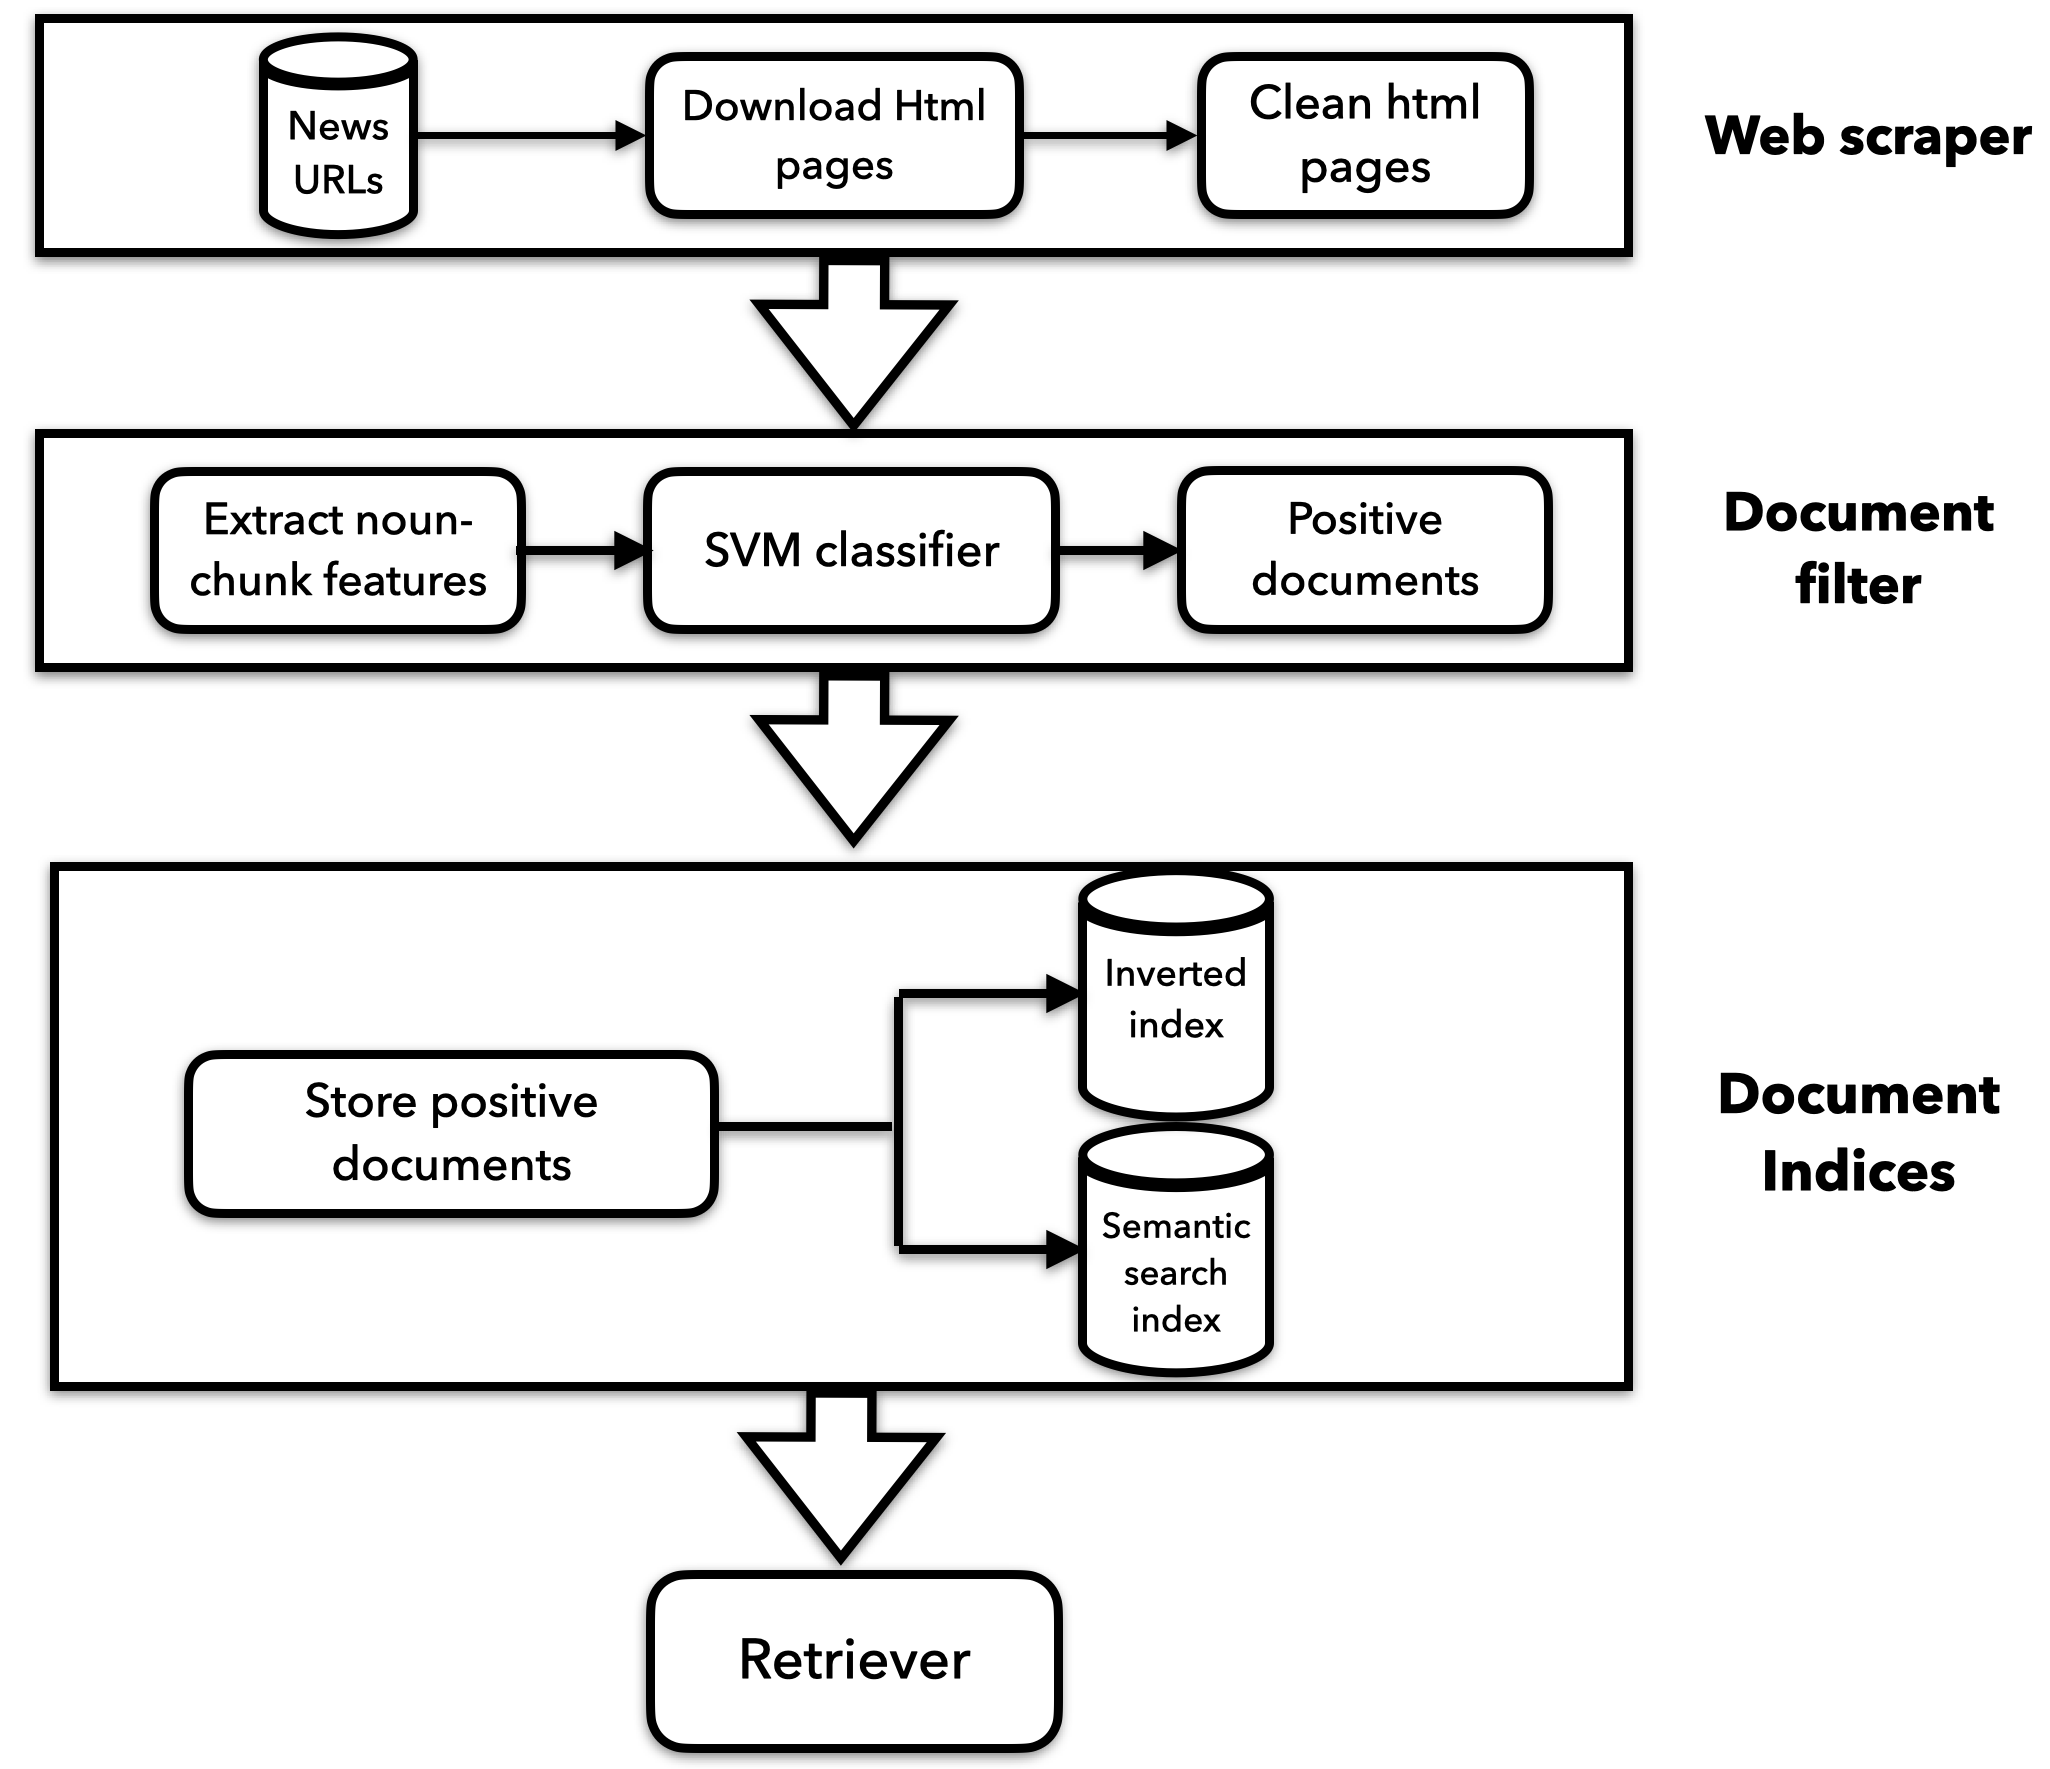
\includegraphics[width=.9\textwidth]{images/thesis_images/background.png}
	\caption[Existing work developed at FKIE.]{Document retrieval system designed at FKIE. \label{fig:background_image}}
\end{figure}

The first component, known as the "Web scraper", retrieves news articles in the form of HTML files from a predefined list of URLs. It then proceeds to clean the raw HTML data by removing advertisements and other irrelevant content. Each cleaned news article is treated as an individual entity referred to as a "Document". The majority of downloaded documents cover a range of topics including military, technology, artificial intelligence, and other typical news subjects like politics, sports, and advertisements. These news articles are available in both German and English.

The second component, referred to as the "Document filter", employs a \ac{SVM} classifier to filter out irrelevant documents that are not related to specific news topics. The documents are classified into two distinct classes: "Positive" and "Negative". Positive documents are news articles related to technology and military topics, while the negative documents cover all other subjects. Various features from different techniques, such as noun chunks, verbs, adjectives, and fine-tuning of \ac{BERT} models, have been evaluated. The results indicate that features derived from noun chunks in a document yield the best performance in distinguishing between positive and negative documents. Noun chunk features based on the pre-trained multi-lingual \ac{USE} are utilized for the classification task.

\begin{figure}[h]
	\centering
	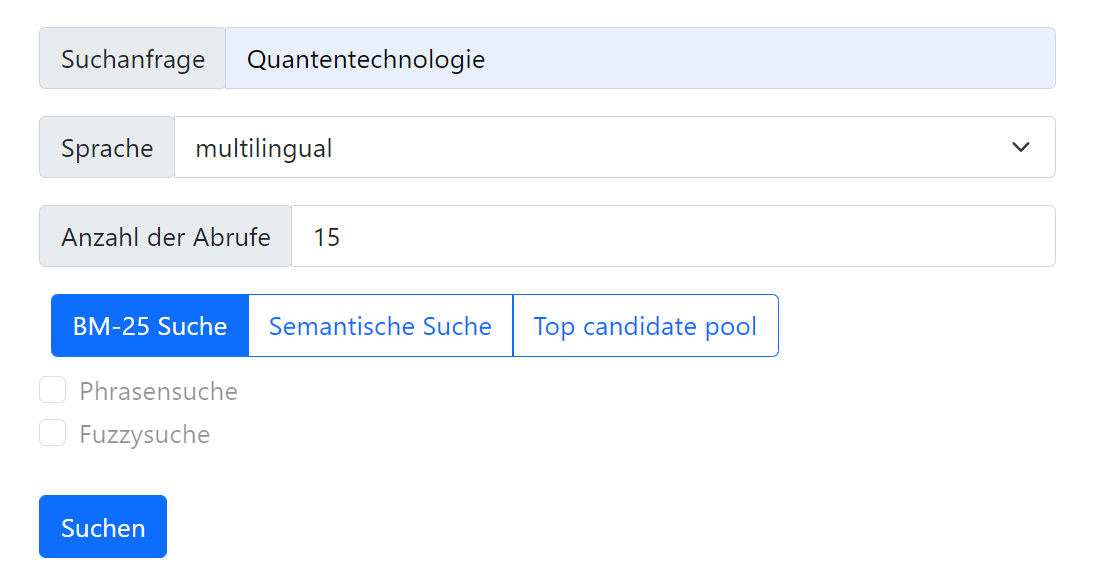
\includegraphics[width=.7\textwidth]{images/mitera_screenshots/newsfeeds_search.PNG}
	\caption[Search user interface.]{User interface to retrieve documents for FKIE users. \label{fig:mitera_search}}
\end{figure}

The positive documents obtained from the "Document filter" stage are stored in two separate document indices, namely the inverted index and the semantic search index (see definitions above and Appendix \ref{appendix:A} for more details). To retrieve documents for a given user query, a dedicated "Retriever" component has been developed, which utilizes both indices and employs lexical and semantic matching techniques. The retrieval process is assisted through a user-friendly web interface, as depicted in \prettyref{fig:mitera_search}. A total of 327,421 news articles were initially scraped, and after applying the document filtering, 26,954 news articles were stored in the document indices. These stored documents are further used in the retrieval process.


\section{Problem Description}

Semantic matching is particularly effective when dealing with long sentence queries due to the contextual information embedded in the search query. For example, a detailed query such as \textit{What are the technological advancements in Robotics related to Unmanned Weapon Systems?} yields high-quality results in the top search results, as it provides specific and comprehensive information requirements. However, in case of keyword queries, semantic and lexical matching approaches tend to generate numerous false positives and offer no significant advantages. This issue of false positives and lack of uniqueness in lexical matching was also observed by Kuzi et al.~\cite{kuzi2020leveraging} in their research.


 Lexical matching does not consider the inherent meaning of the word causing a vocabulary mismatch problem especially in case of polysemy, synonymy. For example, the words "Vehicle," "Automobile," and "Car" essentially refer to the same thing, but lexical matching techniques fail to establish their relationship. Conversely, semantic matching may retrieve a large number of documents that match the query keywords semantically, but it often fails to present the most relevant documents in the top search results. A manual observation of retrieved results is carried out with a set of sample queries to evaluate the retrieval algorithms,and the results are shared in \prettyref{tab:ir_system_comparison}.



\begin{center}
	\captionof{table}[Retrieval algorithms comparison.]{Retrieval algorithms comparison on different query types.}\label{tab:ir_system_comparison}
	\begin{tabularx}{.99\textwidth}{|Y|Y|Y|Y|}
		
		\hline
		  Query type & Better retrieval technique &  Reason &  Queries used  \\
		\hline
	 No meaning queries & BM-25 &  Lexical matching  & Person or object names\footnote{User query with no innate meaning of the word namely out of vocabulary words: for example John Dowe, Wester etc.} \\
		\hline
		 Multi-lingual queries & Semantic search &  Semantic matching & Artificial Intelligence vs Künstliche Intelligenz\\
		\hline
	 German composite words  & Semantic search&  Semantic matching & Quantentechnologie \\
		\hline
	 Spelling mistakes  &  Semantic search&  Semantic matching & Kryptografy, Rbot \\
		\hline
	 Polysemy  & Semantic search&  Semantic matching & Combat Cloud, Cloud computing \\
		\hline
	 Sentence/long phrase queries  & Semantic search&  Semantic matching  & Schwachstell-
		enanalyse eigene Waffen-Systeme \\
		\hline
		
	\end{tabularx}
\end{center}

The users at \ac{FKIE} typically provide concise phrase queries which usually consists of just one or two words. Their intention is to explore information related to specific topics such as "Technology" and "Military". However, learning the user's intention solely based on a single word or phrase query poses a significant challenge in the absence of labeled data. Additionally, another obstacle arises from the diverse range of information sources, which can result in high levels of noise and an increased likelihood of encountering false positives. As a consequence, users are less likely to find the relevant documents among the top search results. 


\begin{figure}[h]
	\centering
	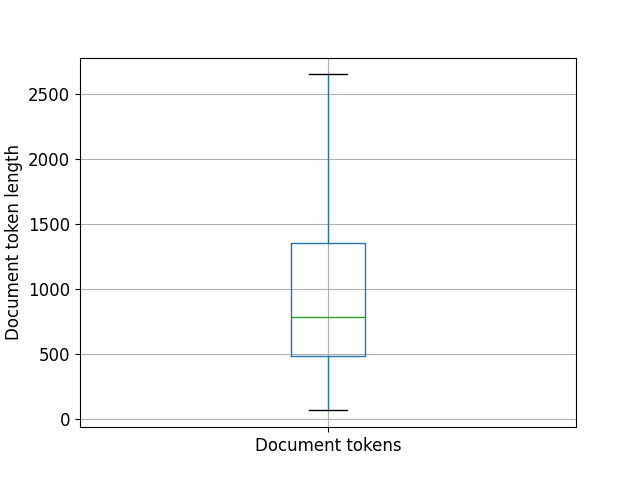
\includegraphics[width=.65\textwidth]{images/keynotes_images/token_length_boxplot.png}
	\caption[Document length distribution.]{Document token length distribution (after removing the outliers). \label{fig:token_length_distribution}}
\end{figure}

Unlike tweets or abstract natural language requirements, news articles are lengthy text documents with a median token length of 788 and encompass keywords from multiple domains. The distribution of document token lengths is illustrated in \prettyref{fig:token_length_distribution}. Finding information regarding innovation and technological breakthroughs within news articles poses a significant challenge. Information related to innovation and technological breakthroughs is hard to find in the news articles. However, the probability is not zero, as positive news articles are gathered during data collection for classification. Due to these challenges, achieving a supervised solution that can match the performance of a full sentence query is challenging. Real-time user feedback and continuous reinforcement algorithms have the potential to address the lack of labeled datasets. However, they require regular feedback from diverse users to avoid biased results that favor a particular user.



\begin{center}
	\captionof{table}[Clustering results in German and English.]{Clustering results to generate more document representations in German and English.}\label{tab:clustering_100_output}
	\begin{tabularx}{.99\textwidth}{|c|Y|}
		\hline
		Query & Clusters \\
		\hline
		
		Quantentechnologie     & Technologie, Microsoft, Military, KI, Quantenteilchen, Quantum computing, Forschung, Bundesministerium, Quantencomputer, München, Industrie, Netzwerke, Algorithm, Quantencomputing, Ingenieuren Informatiker, Qubit, Programmierung, Marineschiff, Intelligence, China, Verteidigung, IBM, AI, Quantum physic, Wissenschaftler, Electronic, Prozessor, Deutschland, Future, Vorsprung, Robotic, Compute, Memory SSDs, USA, Entwicklung, Raumfahrt, Klima, Cybersicherheit, Stau, Rheinmetall Waffe, Laserstrahl \\  \hline
		
		5G          & 5G, 5G network, Frequenzspektrum, 5G deployment, China, Defence intelligence, Nokia, Berlin, Mobilfunkmast, Telekom, Gigabit speed, 4G, WiFi, UMTS, Military, Fiberoptic broadband, 5G technology, Vodafone, Experimentation testing, Mobilfunknetzbetreiber, Technologie, Netzwerk, LTE, Smartphones, Netz, Aircraft, 5G service, Data cap, Deutsche Telekom, Telefónica, Apple, Gebiet, Netzausbau, Anbieter \\  \hline
		
		
		
	\end{tabularx}
	
\end{center}


One approach to enhance the context of a search query is by utilizing a template-based search query. This involves using a predefined template, such as "Innovations in XXX related to the Military."  When the user provides a query such as "Robotics," the "XXX" in the template is replaced with the user's query, resulting in the final query, "Innovations in Robotics related to Military." This template can be dynamically updated based on the user's interests through the user interface, allowing for customized results without the need for additional training. However, this approach has limitations as it restricts users to a limited set of templates and can be inefficient when adding new templates or updating existing ones.


\mycomment{\begin{center}
		\captionof{table}{Keywords present in one retrieved document for the query Quantentechnologie.}\label{tab:keywords_distinction}
		\begin{tabularx}{.75\textwidth}{|Y|Y|}
			\hline
			Keywords similar to the query & Keywords useful for clustering  \\
			\hline
			
			Quantum Technology \newline technological application \newline quantum system \newline quantum computer \newline quantum communication \newline Quantum application \newline quantum bit \newline Quantum sensing \newline quantum radar \newline quantum physics \newline a quantum computer increase \newline a compute unit  &   Sciences  \newline electronic warfare capability \newline the Defense Science Board \newline nuclear material \newline military \newline encode information \newline military personnel \newline military sensing \newline Military Applications \newline Defense Primer \newline enhanced military capability \newline the National Academy \newline potential military application \newline sea-base nuclear deterrent      \\  \hline
			
			
			
		\end{tabularx}
		
\end{center}

One crucial observation has shown that
some keywords from the documents can be omitted during the clustering to improve the clustering
output by creating diverse clusters and maintaining deep representations.  \prettyref{tab:keywords_distinction} details the keywords similar and dissimilar to the query. This query
similarity can play an essential role in creating unique clusters, and it is evaluated extensively
in this thesis.

}

The documents retrieved for certain queries are organized into clusters based on the terms contained within them, forming pathways to access the retrieved documents. The clustering output shown in \prettyref{tab:clustering_100_output}, demonstrates the selection of parameters to generate more comprehensive representations of the retrieved documents. However, it has been observed that some clusters are repetitive and closely resemble the query resulting in the same set of documents being represented and potentially leading to lower user satisfaction.

\begin{figure}[h]
	\centering
	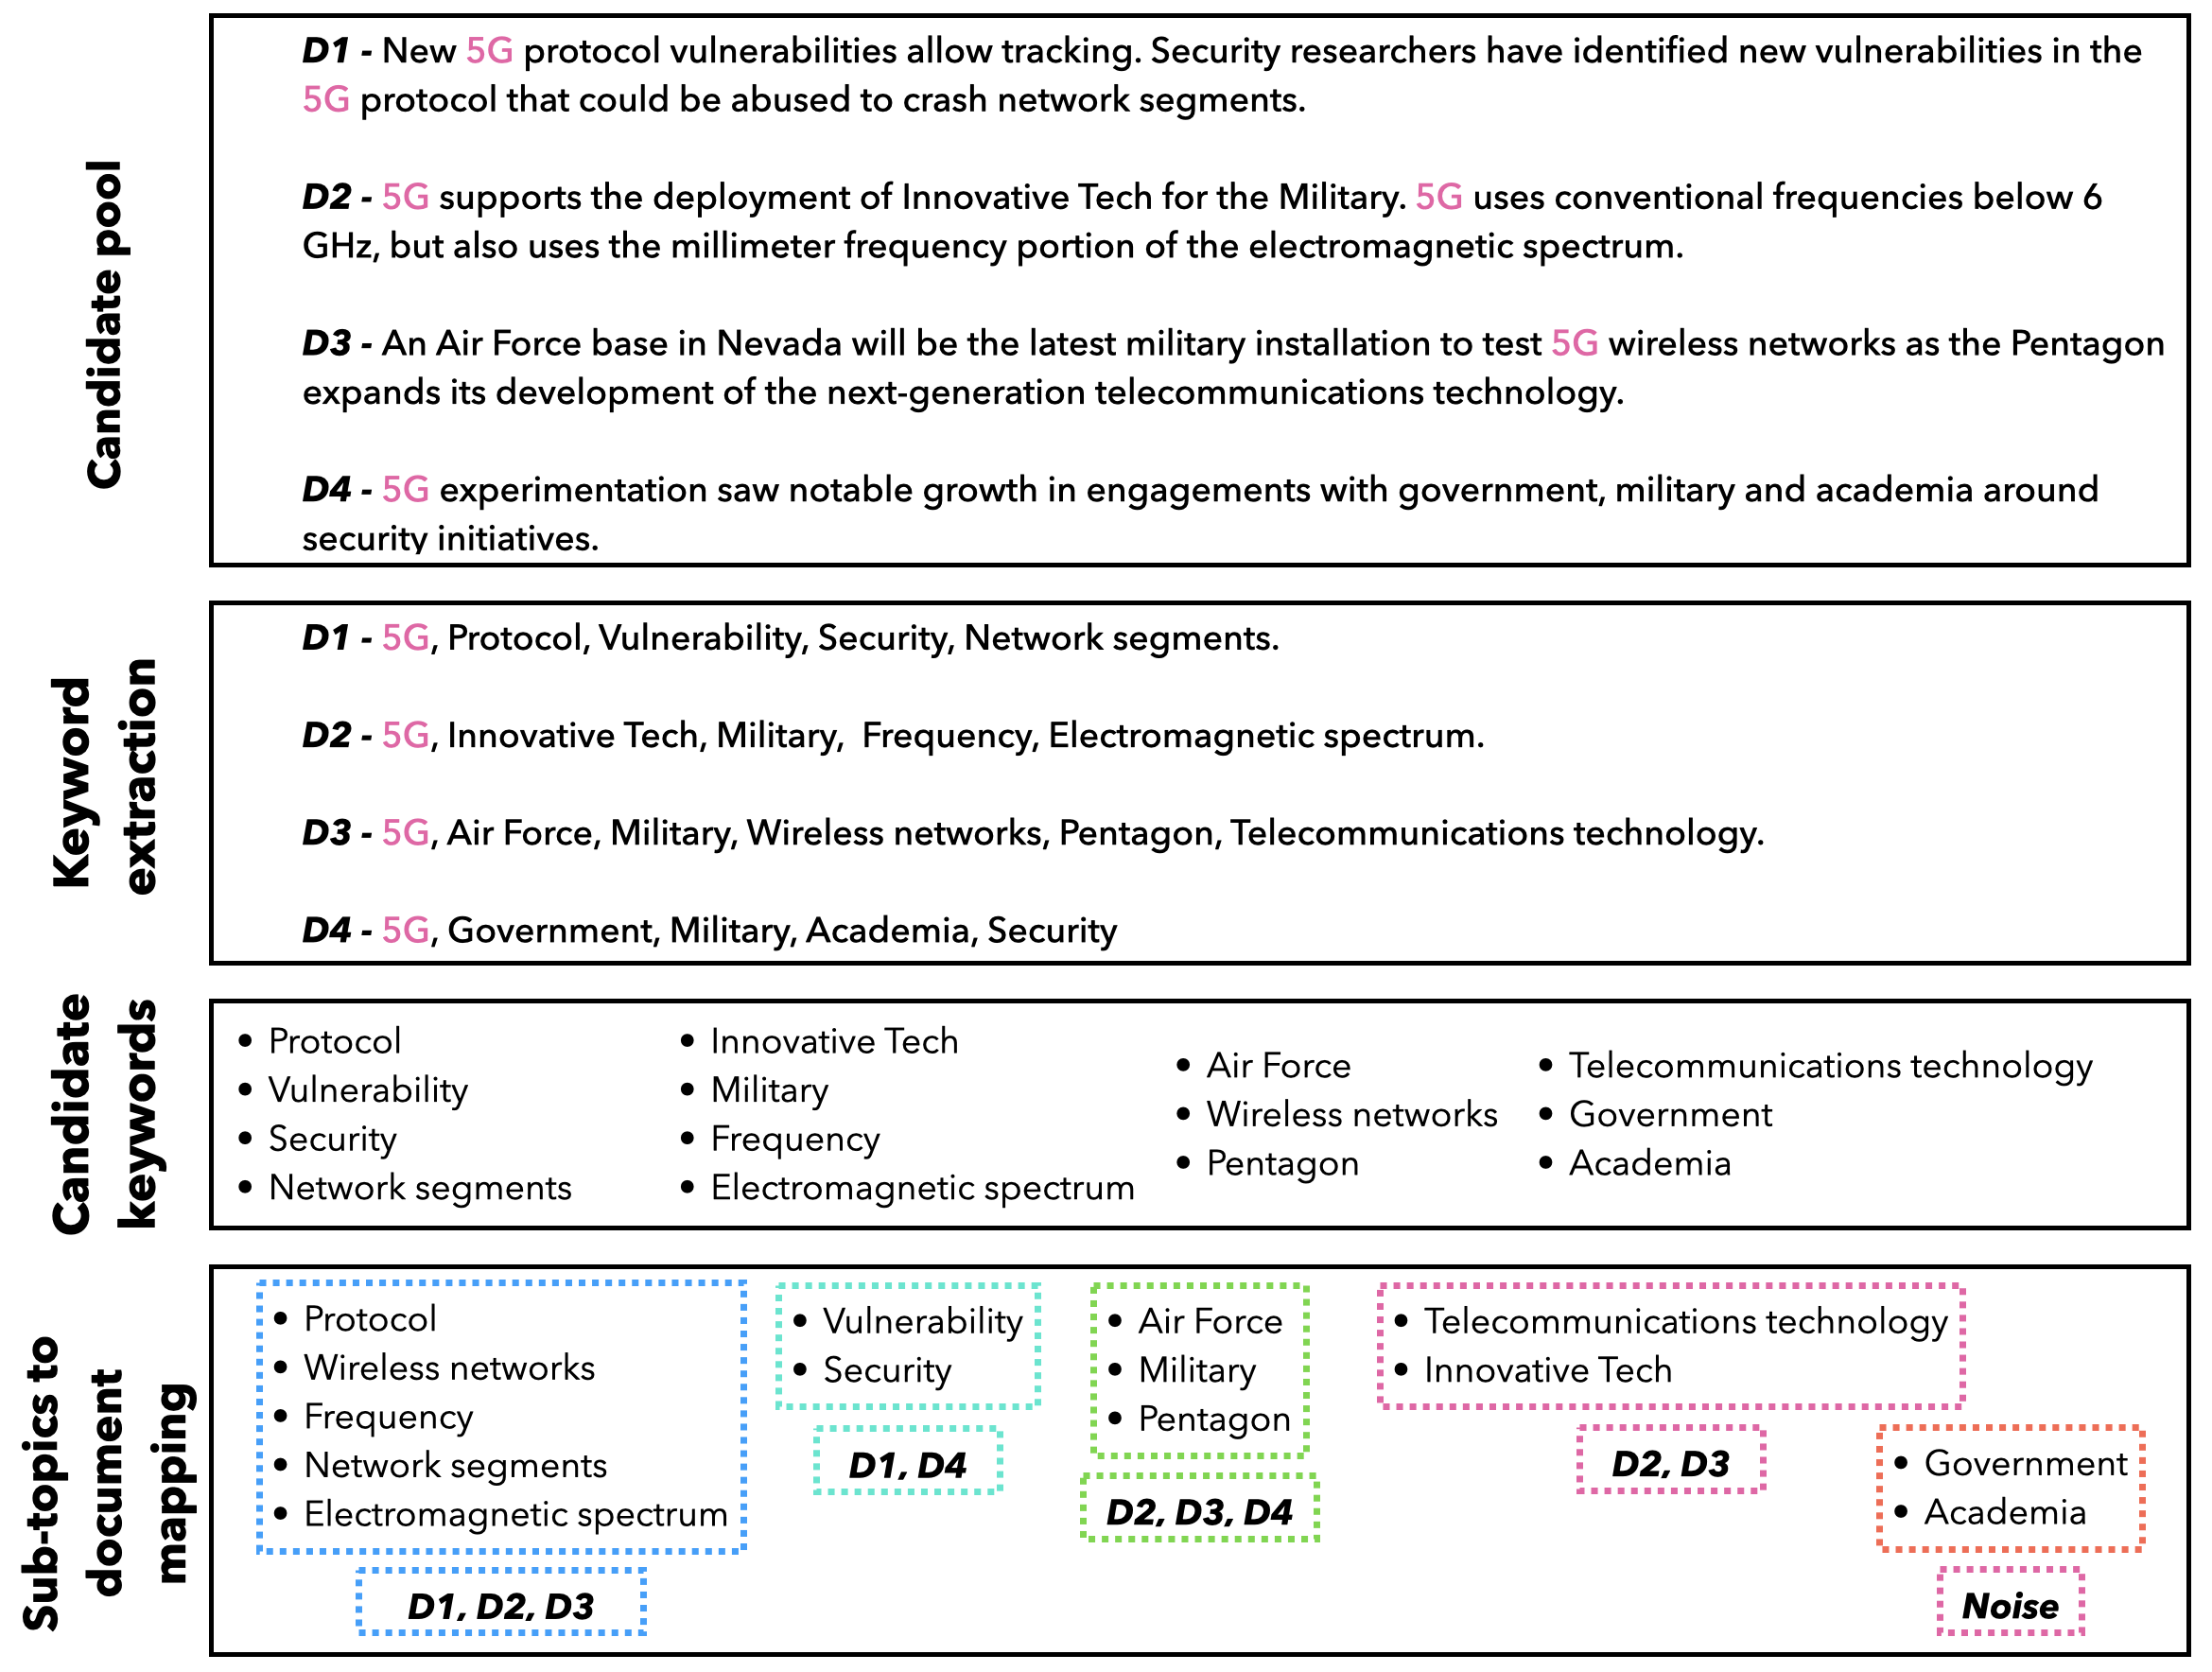
\includegraphics[width=.99\textwidth]{images/keynotes_images/high_level_approach}
	\caption[Expected sub-topic retrieval.]{Expected sub-topic extraction for the query: 5G. \label{fig:proposal_idea}}
\end{figure}

Conversely, selecting parameters that produce fewer representations results in larger individual clusters containing more documents. This, in turn, leads to document repetition within the clusters. After evaluating various approaches to address this issue, it is observed that extracting unique contexts in an unsupervised manner from the top results of a user query is more efficient, explainable, and reproducible compared to supervised approaches. This approach not only provides users with deeper insights into the results but also reduces the effort required to find highly relevant documents. 

\prettyref{fig:proposal_idea} presents a sample output of the expected context extraction pipeline, where the extracted unique contexts are referred to as "sub-topics". The proposed approach in this master thesis aims to tackle the aforementioned challenges and generate highly diverse sub-topics. It considers news articles from diverse sources and can be easily adapted to other sources containing long text documents.



